% !TeX program = pdflatex
% ---------------------------------------------------------------------------
% Durable7 -- The Persistent Data Structure Field Guide
%
% A single-document tour of every data structure in the Durable7 repository.
%
% Build:  latexmk -pdf durable7-data-structures.tex
%
% SPDX-License-Identifier: MIT-0
% ---------------------------------------------------------------------------

\documentclass[11pt,twoside,openright]{book}

% --- Encoding, language, fonts --------------------------------------------
\usepackage[T1]{fontenc}
\usepackage[utf8]{inputenc}
\usepackage[english]{babel}
\usepackage{libertinus}
\usepackage[varqu,varl,scaled=0.95]{inconsolata}
\usepackage{microtype}
\usepackage{textcomp}

% --- Page geometry ---------------------------------------------------------
\usepackage[
  paperwidth=7in, paperheight=9.25in,
  inner=0.95in, outer=0.78in,
  top=0.95in, bottom=1.05in,
  headsep=16pt, footskip=30pt
]{geometry}

% --- Graphics, colour, boxes ----------------------------------------------
\usepackage[table]{xcolor}
\usepackage{tikz}
\usetikzlibrary{arrows.meta,positioning,calc,fit,backgrounds,shapes.geometric,
                decorations.pathreplacing,decorations.pathmorphing,patterns}
\usepackage[most]{tcolorbox}
\tcbuselibrary{skins,breakable}
\usepackage{booktabs}
\usepackage{tabularx}
\usepackage{array}
\usepackage{longtable}
\usepackage{enumitem}
\usepackage{listings}
\usepackage{caption}
\usepackage{float}
\usepackage{needspace}
\usepackage{makeidx}
\makeindex

% --- Palette ---------------------------------------------------------------
\definecolor{d7ink}      {HTML}{16243C} % deep navy -- headings, body accents
\definecolor{d7copper}   {HTML}{A8562B} % warm accent -- rules, caveats
\definecolor{d7teal}     {HTML}{176E6E} % cool accent -- links, contracts
\definecolor{d7slate}    {HTML}{5A6779} % muted text
\definecolor{d7rule}     {HTML}{C9CFDA} % hairlines
\definecolor{d7paper}    {HTML}{F7F5F0} % box fill, warm
\definecolor{d7mist}     {HTML}{EEF2F6} % box fill, cool
\definecolor{d7sun}      {HTML}{F6EEE2} % box fill, caveat
\definecolor{d7leaf}     {HTML}{3E6B4A} % code strings
\definecolor{d7plum}     {HTML}{6B3A6B} % code keywords 2

% --- Hyperlinks ------------------------------------------------------------
\usepackage[
  colorlinks=true,
  linkcolor=d7ink,
  urlcolor=d7teal,
  citecolor=d7teal,
  pdftitle={Durable7: The Persistent Data Structure Field Guide},
  pdfauthor={The Durable7 Project},
  pdfsubject={Persistent and authenticated data structures},
  pdfkeywords={persistent data structures, CHAMP, HAMT, finger tree, RRB vector,
               Merkle search tree, zip tree, Patricia trie, rope},
  bookmarksnumbered=true,
  bookmarksopen=true,
  bookmarksopenlevel=1
]{hyperref}
\usepackage{bookmark}

% --- Sectioning style ------------------------------------------------------
\usepackage[explicit]{titlesec}

\titleformat{\part}[display]
  {\normalfont\sffamily\filcenter}
  {\color{d7copper}\large\scshape\partname~\thepart}
  {14pt}
  {\color{d7ink}\Huge\bfseries #1}
  [\vspace{10pt}{\color{d7copper}\rule{2.2cm}{1.4pt}}]

\titleformat{\chapter}[display]
  {\normalfont\sffamily}
  {\raggedleft\color{d7rule}\fontsize{62}{62}\selectfont\bfseries\thechapter}
  {-8pt}
  {\raggedright\color{d7ink}\huge\bfseries #1}
  [\vspace{7pt}{\color{d7copper}\rule{\textwidth}{1.1pt}}]
\titlespacing*{\chapter}{0pt}{-24pt}{28pt}

\titleformat{name=\chapter,numberless}[display]
  {\normalfont\sffamily}
  {}
  {0pt}
  {\raggedright\color{d7ink}\huge\bfseries #1}
  [\vspace{7pt}{\color{d7copper}\rule{\textwidth}{1.1pt}}]

\titleformat{\section}
  {\normalfont\sffamily\Large\bfseries\color{d7ink}}
  {\color{d7copper}\thesection}{0.7em}{#1}
\titleformat{\subsection}
  {\normalfont\sffamily\large\bfseries\color{d7ink}}
  {\color{d7copper}\thesubsection}{0.6em}{#1}
\titleformat{\subsubsection}
  {\normalfont\sffamily\normalsize\bfseries\color{d7slate}}
  {}{0pt}{#1}
\titlespacing*{\section}{0pt}{18pt plus 4pt minus 2pt}{7pt}
\titlespacing*{\subsection}{0pt}{14pt plus 3pt minus 2pt}{5pt}

% --- Running heads ---------------------------------------------------------
\usepackage{fancyhdr}
\fancypagestyle{d7main}{%
  \fancyhf{}
  \renewcommand{\headrulewidth}{0pt}
  \fancyhead[LE]{\sffamily\footnotesize\color{d7slate}\thepage\quad\textbar\quad\leftmark}
  \fancyhead[RO]{\sffamily\footnotesize\color{d7slate}\rightmark\quad\textbar\quad\thepage}
}
\fancypagestyle{plain}{%
  \fancyhf{}
  \renewcommand{\headrulewidth}{0pt}
  \fancyfoot[C]{\sffamily\footnotesize\color{d7slate}\thepage}
}
\renewcommand{\chaptermark}[1]{\markboth{\textsc{\lowercase{#1}}}{}}
\renewcommand{\sectionmark}[1]{\markright{\textsc{\lowercase{#1}}}}
\pagestyle{d7main}

% --- Typographic details ---------------------------------------------------
\setlength{\parskip}{0pt}
\setlength{\parindent}{1.2em}
\linespread{1.06}
\setlist{itemsep=2pt,parsep=1pt,topsep=5pt}
\setlist[itemize]{label=\textcolor{d7copper}{\small$\blacktriangleright$}}
\setlist[description]{font=\sffamily\bfseries\color{d7ink}}
\captionsetup{font=small,labelfont={sf,bf,color=d7copper},textfont={color=d7slate},
              justification=raggedright,singlelinecheck=false}
\renewcommand{\arraystretch}{1.18}
\arrayrulecolor{d7rule}

% --- Inline helpers --------------------------------------------------------
\newcommand{\code}[1]{\texorpdfstring{\textcolor{d7ink}{\texttt{#1}}}{#1}}
\newcommand{\lang}[1]{\textsf{\small #1}}
\newcommand{\term}[1]{\textit{#1}}
\newcommand{\bigoh}[1]{$\mathrm{O}(#1)$}

% Chapter epigraph
\newcommand{\epigraph}[2]{%
  \begingroup
  \vspace{-6pt}\hfill\begin{minipage}{0.82\textwidth}
    \raggedleft\itshape\color{d7slate}\small #1\par
    \vspace{3pt}\normalfont\sffamily\scriptsize\upshape --- #2\par
  \end{minipage}\par\vspace{16pt}
  \endgroup}

% --- Code listings ---------------------------------------------------------
\lstdefinelanguage{Rust}{
  morekeywords={as,async,await,break,const,continue,crate,dyn,else,enum,extern,
    false,fn,for,if,impl,in,let,loop,match,mod,move,mut,pub,ref,return,self,Self,
    static,struct,super,trait,true,type,unsafe,use,where,while},
  morekeywords=[2]{Arc,Rc,Option,Result,Some,None,Ok,Err,Vec,String,usize,u32,u64,
    i32,i64,bool,str,Clone,Eq,Hash,BuildHasher,Send,Sync},
  sensitive=true, morecomment=[l]{//}, morecomment=[s]{/*}{*/}, morestring=[b]",
}
\lstdefinelanguage{TypeScript}{
  morekeywords={as,async,await,break,case,catch,class,const,continue,default,
    delete,do,else,export,extends,false,finally,for,from,function,if,implements,
    import,in,instanceof,interface,let,new,null,of,readonly,return,static,super,
    switch,this,throw,true,try,type,typeof,undefined,var,void,while,yield},
  morekeywords=[2]{string,number,boolean,bigint,unknown,never,any,Map,Set,Array,
    Promise,Iterable,Readonly},
  sensitive=true, morecomment=[l]{//}, morecomment=[s]{/*}{*/},
  morestring=[b]",morestring=[b]',
}
\lstdefinelanguage{Kotlin}{
  morekeywords={as,break,by,class,companion,const,continue,data,do,else,enum,
    false,for,fun,if,in,init,interface,internal,is,null,object,open,operator,
    override,package,private,public,return,sealed,super,this,throw,true,try,
    val,var,vararg,when,while},
  morekeywords=[2]{Int,Long,String,Boolean,List,Map,Set,Any,Unit,Nothing},
  sensitive=true, morecomment=[l]{//}, morecomment=[s]{/*}{*/},
  morestring=[b]",morestring=[b]',
}

\lstdefinestyle{d7}{
  basicstyle=\ttfamily\footnotesize\color{d7ink},
  keywordstyle=\color{d7ink}\bfseries,
  keywordstyle=[2]\color{d7plum},
  commentstyle=\itshape\color{d7slate},
  stringstyle=\color{d7leaf},
  showstringspaces=false,
  breaklines=true,
  breakatwhitespace=true,
  breakindent=1.6em,
  postbreak=\mbox{\textcolor{d7copper}{$\hookrightarrow$}\space},
  columns=fullflexible,
  keepspaces=true,
  tabsize=2,
  frame=leftline,
  framerule=1.4pt,
  rulecolor=\color{d7rule},
  framesep=9pt,
  xleftmargin=11pt,
  aboveskip=11pt,
  belowskip=8pt,
  upquote=true,
}
\lstset{style=d7}

% --- Callout boxes ---------------------------------------------------------
\newtcolorbox{contractbox}[1][The contract]{
  enhanced, breakable,
  colback=d7mist, colframe=d7teal,
  boxrule=0pt, leftrule=2.6pt,
  arc=0pt, outer arc=0pt,
  left=10pt, right=10pt, bottom=8pt, top=14pt,
  fonttitle=\sffamily\bfseries\footnotesize,
  coltitle=d7teal,
  title={\MakeUppercase{#1}},
  attach boxed title to top left={xshift=10pt, yshift=-2pt},
  boxed title style={colback=d7mist, boxrule=0pt, arc=0pt, left=2pt, right=2pt},
}
\newtcolorbox{caveatbox}[1][Caveat]{
  enhanced, breakable,
  colback=d7sun, colframe=d7copper,
  boxrule=0pt, leftrule=2.6pt,
  arc=0pt, outer arc=0pt,
  left=10pt, right=10pt, top=14pt, bottom=8pt,
  fonttitle=\sffamily\bfseries\footnotesize,
  coltitle=d7copper,
  title={\MakeUppercase{#1}},
  attach boxed title to top left={xshift=10pt, yshift=-2pt},
  boxed title style={colback=d7sun, boxrule=0pt, arc=0pt, left=2pt, right=2pt},
}
\newtcolorbox{glancebox}[1][At a glance]{
  enhanced, breakable,
  colback=white, colframe=d7rule,
  boxrule=0.8pt,
  arc=2pt, outer arc=2pt,
  left=11pt, right=11pt, top=15pt, bottom=9pt,
  fonttitle=\sffamily\bfseries\footnotesize,
  coltitle=d7slate,
  title={\MakeUppercase{#1}},
  attach boxed title to top left={xshift=11pt, yshift=-7pt},
  boxed title style={colback=white, boxrule=0pt, arc=0pt, left=3pt, right=3pt},
}
\newtcolorbox{asidebox}[1][Aside]{
  enhanced, breakable,
  colback=d7paper, colframe=d7paper,
  boxrule=0pt, arc=2pt,
  left=12pt, right=12pt, top=14pt, bottom=9pt,
  fonttitle=\sffamily\bfseries\footnotesize,
  coltitle=d7slate,
  title={\MakeUppercase{#1}},
  attach boxed title to top left={xshift=12pt, yshift=-2pt},
  boxed title style={colback=d7paper, boxrule=0pt, arc=0pt, left=2pt, right=2pt},
}

% A compact "specimen card" used to open each structure's section.
\newenvironment{specimen}[1][Specimen]
  {\begin{glancebox}[#1]\small
   \setlength{\tabcolsep}{4pt}\renewcommand{\arraystretch}{1.14}
   \begin{tabularx}{\linewidth}{@{}>{\sffamily\bfseries\color{d7slate}\footnotesize\raggedright\arraybackslash}p{0.21\linewidth}X@{}}}
  {\end{tabularx}\end{glancebox}}

% Table helpers
\newcolumntype{L}[1]{>{\raggedright\arraybackslash}p{#1}}
\newcolumntype{Y}{>{\raggedright\arraybackslash}X}
\newcommand{\thead}[1]{\sffamily\bfseries\footnotesize\color{d7ink}#1}

% TikZ shared styles
\tikzset{
  d7node/.style={draw=d7ink, fill=white, rounded corners=1.5pt, inner sep=3pt,
                 font=\sffamily\scriptsize, minimum height=15pt},
  d7leafnode/.style={d7node, fill=d7mist},
  d7newnode/.style={d7node, draw=d7copper, fill=d7sun, very thick},
  d7ghost/.style={d7node, draw=d7rule, text=d7slate},
  d7edge/.style={-{Stealth[length=4pt]}, draw=d7slate, thin},
  d7newedge/.style={-{Stealth[length=4pt]}, draw=d7copper, thick},
  d7label/.style={font=\sffamily\scriptsize\color{d7slate}},
  d7cell/.style={draw=d7slate, thin, minimum width=13pt, minimum height=13pt,
                 font=\ttfamily\tiny, inner sep=0pt},
}

\begin{document}
\frenchspacing

% ===========================================================================
%  FRONT MATTER
% ===========================================================================
\frontmatter
\pagestyle{empty}

% --- Title page ------------------------------------------------------------
\begin{titlepage}
\centering
\vspace*{0.10\textheight}

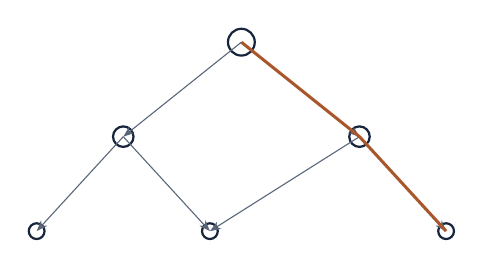
\begin{tikzpicture}[scale=1]
  % A stylised "version DAG": one root, three shared branches.
  \definecolor{c}{HTML}{16243C}
  \foreach \x/\y/\r in {0/0/3.4, -1.5/-1.2/2.6, 1.5/-1.2/2.6,
                        -2.6/-2.4/2.0, -0.4/-2.4/2.0, 2.6/-2.4/2.0}
    { \node[circle, draw=d7ink, fill=white, line width=0.8pt,
            minimum size=\r mm, inner sep=0pt] at (\x,\y) {}; }
  \draw[d7edge] (0,0) -- (-1.5,-1.2);
  \draw[d7edge] (0,0) -- (1.5,-1.2);
  \draw[d7edge] (-1.5,-1.2) -- (-2.6,-2.4);
  \draw[d7edge] (-1.5,-1.2) -- (-0.4,-2.4);
  \draw[d7edge] (1.5,-1.2) -- (-0.4,-2.4);
  \draw[d7edge] (1.5,-1.2) -- (2.6,-2.4);
  \draw[d7copper, line width=1.1pt] (0,0) -- (1.5,-1.2) -- (2.6,-2.4);
\end{tikzpicture}

\vspace{0.05\textheight}

{\sffamily\fontsize{13}{16}\selectfont\color{d7copper}\scshape
 The Durable7 Field Guide\par}

\vspace{14pt}
{\color{d7copper}\rule{0.34\textwidth}{1.2pt}}
\vspace{18pt}

{\sffamily\fontsize{34}{40}\selectfont\bfseries\color{d7ink}
 Persistent\\Data Structures\par}

\vspace{16pt}

{\sffamily\fontsize{14}{20}\selectfont\color{d7slate}
 Nine languages, one contract,\\forty-odd immutable collections\par}

\vspace{0.16\textheight}

{\sffamily\small\color{d7slate}
 A complete tour of the collections in the\\
 \textbf{Durable7} repository --- what each one is,\\
 why it exists, and when to reach for it.\par}

\vfill
{\sffamily\footnotesize\color{d7slate}
 Pre-release 0.1.0 \quad\textbullet\quad MIT No Attribution\par}
\end{titlepage}

% --- Colophon --------------------------------------------------------------
\thispagestyle{empty}
\null\vfill
\begin{flushleft}\small\color{d7slate}
\textbf{\sffamily Durable7: The Persistent Data Structure Field Guide}\\[6pt]
This document describes the collections implemented in the Durable7 repository.
It is a companion to --- not a replacement for --- the workspace API
specifications and public headers, which remain the normative source for
contracts, complexity, allocation behaviour, and validation evidence.
Where this guide and a workspace specification disagree, the specification
wins and this guide has a bug.\\[10pt]
The repository ports every family to \textbf{C}, \textbf{C\texttt{++}},
\textbf{C\#}, \textbf{Haskell}, \textbf{Kotlin}, \textbf{OCaml},
\textbf{Python}, \textbf{Rust}, and \textbf{TypeScript}. Code samples are drawn
from whichever port makes the point most clearly; every behaviour described in
the shared-contract sections holds in all nine unless the text says
otherwise.\\[10pt]
Set in Libertinus with Inconsolata for code; diagrams drawn in \textsc{Ti\emph{k}Z};
typeset with \LaTeX.\\[10pt]
Licensed \textbf{MIT No Attribution (MIT-0)}. Use it, fork it, ship it.
\end{flushleft}
\vspace{18pt}

% --- Contents --------------------------------------------------------------
\cleardoublepage
\pagestyle{plain}
\setcounter{tocdepth}{1}
{\hypersetup{linkcolor=d7ink}
 \renewcommand{\contentsname}{Contents}
 \tableofcontents}

% --- How to read -----------------------------------------------------------
\cleardoublepage
\pagestyle{d7main}
\chapter*{How to read this guide}
\addcontentsline{toc}{chapter}{How to read this guide}
\markboth{\textsc{how to read this guide}}{\textsc{how to read this guide}}

There are two honest ways to use a book about data structures. You can read it
straight through, which is what you want when you are trying to understand a
design space. Or you can open it at the one page that answers today's question,
which is what you want at 4pm on a Thursday. This guide is arranged so that both
work.

\bigskip
\noindent\textbf{\sffamily\color{d7ink}If you are reading straight through.}
Part~\ref{part:foundations} explains what persistence buys and what it costs,
and sets out the vocabulary that the rest of the book leans on --- policies,
representatives, no-op identity, failure atomicity. Nothing after it will quite
land without it. Parts~\ref{part:hash} through~\ref{part:authenticated} then walk
the families in the order a curious reader would want them: the hash trie first
(it is the substrate for a third of everything else), then sequences, then
ordered and priority collections, then the authenticated tier. Part~\ref{part:navigation}
covers cursors, which cut across every family. The appendices are reference
material.

\bigskip
\noindent\textbf{\sffamily\color{d7ink}If you are looking something up.}
Every structure gets a \emph{specimen card} --- a compact panel with its purpose,
its complexity, its policy requirements, and its nine-language spellings ---
followed by prose that explains the representation and the decisions inside it.
Appendix~\ref{app:complexity} is a single sorted complexity table across the
whole library. Appendix~\ref{app:names} is a name-to-name index across the nine
ports. The subject index at the back covers both concepts and identifiers.

\bigskip
\noindent\textbf{\sffamily\color{d7ink}Three kinds of panel appear throughout.}

\begin{contractbox}[The contract]
Normative behaviour that every port upholds. If a port cannot honour one of
these, it says so explicitly in its own API notes rather than quietly differing.
\end{contractbox}

\begin{caveatbox}[Caveat]
The place where a claim stops being true. These are the paragraphs worth reading
twice --- most production surprises with persistent structures live exactly at
the edge of an amortisation argument or a policy assumption.
\end{caveatbox}

\begin{asidebox}[Aside]
History, provenance, and the occasional road not taken. Skippable, but they are
where the design reasoning usually hides.
\end{asidebox}

\bigskip
\noindent\textbf{\sffamily\color{d7ink}A note on honesty.} This library is
unusually careful about the difference between a bound it can prove and a bound
it would like to have. Several structures ship as \emph{checkpoints}: the
observable semantics match the reference port exactly, but the representation is
simpler and the asymptotic claim is weaker. Wherever that is the case, this
guide says so in the same breath as the feature. A guide that only reported the
good news would be a worse guide.

%%APPEND-HERE%%

\end{document}
